\chapter{The Elementary Shortest Path Problem with Resource Constraints}
In this chapter we will introduce more formally the Elementary Shortest Path Problem with Resource Constraints (ESPPRC).
In this thesis we're interested in studying the ESPPRC induced from the PP when solving the RMP through a BAP framework employing the usage of robust inequalities only.

In the general case, the underlying network of ESPPRC problems may have negative cost cyles, which makes solving the ESPPRC an NP-hard problem \parencite{dror1994}.

As claimed in \textcite{dror1994}, the ESPPRC is an NP-hard problem,
However, the subproblem can be solved through a dynamic programming approach, as proposed by \textcite{feillet2004}.
The proposed algorithm is a natural extension of the Bellman–Ford algorithm \parencite{bellman1958, fordjr1956},
a common algorithm present in the "toolbelt" of all operations research practicioner,
which computes shortest paths from a source vertex to all other vertices,
by taking also in consideration additional path constraints.

\begin{comment}
\cite{bettinelli2010mathematical} ---------------
It is possible to address the pricing problem by optimizing its relaxation,
obtained by dropping the elementarity constraints. Solving a resource con-
strained shortest path problem (RCSPP) requires less computing time but
yields less tight lower bounds, since columns may include cycles. The two
different approaches have been followed for instance by Feillet et al. [42] and
Desrochers et al. [29] to solve the vehicle routing problem with time windows
(VRPTW) through column generation.
\end{comment}

\section{ESPPRC: IP formulation}
Contrary to CVRP, the ESPPRC is usually defined over a directed network $G^\prime = (V^\prime, A^\prime)$ composed
of $N + 1$ nodes where the original depot node is essentially split in two nodes: a source and a sink vertex.
In the new network we use the value $0$ to denote the source version of the depot node, and $N$ its duplicate
playing the role of the sink vertex.
More formally, $V^\prime = V \cup \Set*{N} = \Set*{ 0,\dots, N }$, and the edge set $A^\prime$ is

\begin{equation}
	\begin{aligned}
		A^\prime = \  & \Set*{(i, j) \mid i, j \in V,\ i \ne j}                       \\
		              & \setminus \Set*{ \Tuple*{0, N} }                              \\
		              & \setminus \Set*{ \Tuple*{i, 0} \quad \forall i \in V^\prime } \\
		              & \setminus \Set*{ \Tuple*{N, i} \quad \forall i \in V^\prime } \\
	\end{aligned}
\end{equation}

which briefly means: all possible pairs $\Tuple*{i, j},\ i \ne j$ excluding: direct connection between $0$ and $N$, and by excluding edges entering node $0$ and flowing out of node $N$.
The edge set $A^\prime$ has size $|A^\prime| = N(N - 1) + 2(N - 1)$.

We use $\deltaplus(S) = \Set*{(i, j) \in A^\prime \mid i \in S, j \notin S}$ to denote the out-arcs crossing the set $S \subset V^\prime$.
We use $\deltaminus(S) = \Set*{(i, j) \in A^\prime \mid i \notin S, j \in S}$ to denote the in-arcs crossing the set $S \subset V^\prime$.
For brevity, we also define $\deltaplus(i) = \deltaplus(\Set*{i})$, $\deltaminus(i) = \deltaminus(\Set*{i})$
to denote respectively the singleton version of the in and out arcs for vertices $i \in V$.

At each directed edge $\Tuple*{i, j} \in A^\prime$ we have an associated weight $\bar{c_{ij}} \in \R$ which is directly linked to the dual variables of the RMP through the following equation:

\begin{equation}
	\bar{c_{ij}} = d_{ij} - \frac{\pi_i + \pi_j}{2} \quad \forall i, j \in V^\prime
\end{equation}

where $\pi$ represent the dual variables associated to constraints \eqref{eq:mp-customers-visited-by-exactly-one-route}\eqref{eq:mp-K-routes},
as was already explained in Section \ref{sec:column-generation-and-pricing-problem}.

Let $x_{ij} \in \Set*{0, 1} \quad \forall i, j \in V^\prime$ be a new set of binary variables
encoding feasible solutions for the ESPRCC problem (i.e. $x_{ij} = 1$ if edge $(i, j)$ is picked in the optimal path).
We can finally write the full ESPPRC IP formulation as:

\begin{align}
	\min_{x} \quad z_\mt{ESPPRC}(x) & =  \sum_{(i, j) \in A^\prime} \bar{c_{ij}} x_{ij} \label{eq:espprc-obj-function}                                                                                                               \\
	                                & \sum_{i \in V_0} \frac{q_i}{2} \Expr*{ \ExprESPPIngoingEdges{i} + \ExprESPPOutgoingEdges{i} }  \le Q                            \label{eq:espprc-resource-upper-bound-constraint}              \\
	                                & \ExprESPPIngoingEdges{i} = \ExprESPPOutgoingEdges{i}                                                \qquad \forall i \in V_0          \label{eq:espprc-flow-conservation-constraint-customers} \\
	                                & \ExprESPPOutgoingEdges[i]{0} = 1                                                                                                      \label{eq:espprc-flow-conservation-constraint-depot1}    \\
	                                & \ExprESPPIngoingEdges[i]{N} = 1                                                                                                       \label{eq:espprc-flow-conservation-constraint-depot2}    \\
	                                & \ExprESPPEdgesWithin[S] \le |S| - 1                                                                  \qquad \forall S \subseteq V^\prime,\ |S| \ge 2 \label{eq:espprc-sec-constraints}         \\
	                                & x_{0i} + x_{iN} \le 1                                                                                \qquad \forall i \in V_0         \label{eq:espprc-binding-directed}                       \\
	                                & x_{ij}                   \in \lbrace 0, 1 \rbrace                                                    \qquad \forall \Tuple*{i, j} \in A^\prime    \label{eq:espprc-x-mip-var-bounds}           \\
\end{align}

where, \eqref{eq:espprc-obj-function} is the objective function which we aim to minimize.
The remaining constraints characterize the set of feasible paths $P$, by paying attention that we are now dealing with
a directed network, and the depot node is duplicated twice.
Namely, constraint \eqref{eq:espprc-resource-upper-bound-constraint} expresses the resource bound modeled as a function of only the $x$ MIP variables,
constraint \eqref{eq:espprc-flow-conservation-constraint-customers} imposes a flow conservation for all vertices excluding the source and the sink node,
constraint \eqref{eq:espprc-flow-conservation-constraint-depot1}, \eqref{eq:espprc-flow-conservation-constraint-depot2} are the flow imposition for respectively the source and sink node,
constraint  \eqref{eq:espprc-binding-directed} avoids forming paths where a single customer is visited, this constraint is a direct consequence of the fact that the CVRP is defined over an undirected network,
constraint \eqref{eq:espprc-x-mip-var-bounds} imposes bound and integrality constraints on the $x$ MIP variables.

Finally, the most important inequalities, constraint \eqref{eq:espprc-sec-constraints}, represents the subtour elimination constraints.
These inequalities have two major impacts: first they avoid the form of spurious unconnected subtours, second they force the elementarity condition, namely they impose that each node must be visited at most once.
Two examples depicting respectively a solution containing spurious subtours and a non-elementary solution are provided in Figures \ref{fig:espprc-example-with-spurious-subtours} and \ref{fig:espprc-example-non-elementary-solution}.

\begin{figure}[ht]
	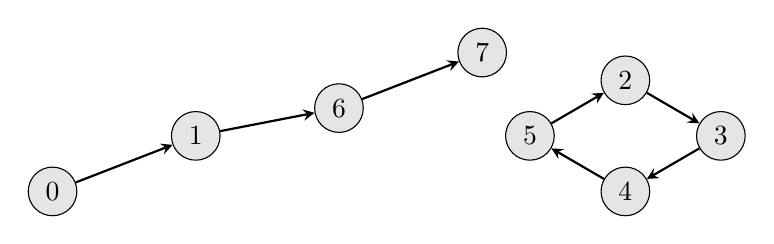
\begin{tikzpicture}[>=stealth, main/.style = {draw, circle, fill=black!10!white}]
		\centering

		\node[main] (0) at (0.1\textwidth,-20bp) {0};
		\node[main] (1) at (0.25\textwidth,0bp){1};
		\node[main] (6) at (0.4\textwidth,+10bp){6};
		\node[main] (7) at (0.55\textwidth,+30bp) {7};

		\node[main] (2) at (0.7\textwidth, +20bp){2};
		\node[main] (3) at (0.8\textwidth, -0bp) {3};
		\node[main] (4) at (0.7\textwidth, -20bp) {4};
		\node[main] (5) at (0.6\textwidth, -0bp) {5};

		\draw [->,thick] (0) -- (1);
		\draw [->,thick] (1) -- (6);
		\draw [->,thick] (6) -- (7);

		\draw [->,thick] (2) -- (3);
		\draw [->,thick] (3) -- (4);
		\draw [->,thick] (4) -- (5);
		\draw [->,thick] (5) -- (2);
	\end{tikzpicture}

	\centering
	\caption{An example of an ESPRRC solution containing spurious subtours.
		$V^\prime = \Set*{0, \dots, 7}$, ($0$ is the source vertex, $7$ the sink vertex).
		SEC inequalities, presented in Equation \eqref{eq:espprc-sec-constraints}, make the situation depicted in the figure impossible to occur.
	}
	\label{fig:espprc-example-with-spurious-subtours}
\end{figure}

\begin{figure}[ht]
	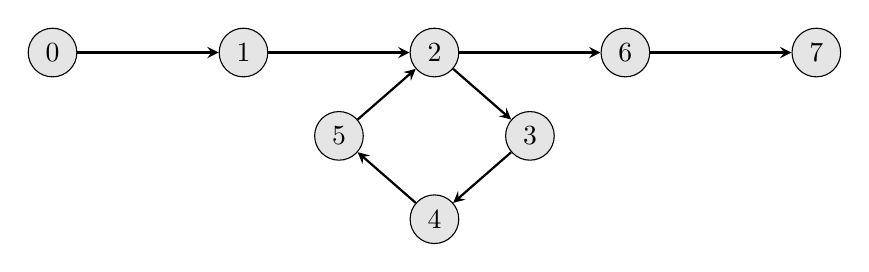
\begin{tikzpicture}[>=stealth, main/.style = {draw, circle, fill=black!10!white}]
		\centering

		\node[main] (0) at (0.1\textwidth,0bp) {0};
		\node[main] (1) at (0.3\textwidth,0bp){1};
		\node[main] (2) at (0.5\textwidth,0bp){2};
		\node[main] (3) at (0.6\textwidth,-30bp) {3};
		\node[main] (4) at (0.5\textwidth,-60bp) {4};
		\node[main] (5) at (0.4\textwidth,-30bp) {5};
		\node[main] (6) at (0.7\textwidth,0bp){6};
		\node[main] (7) at (0.9\textwidth,0bp) {7};

		\draw [->,thick] (0) -- (1);
		\draw [->,thick] (1) -- (2);
		\draw [->,thick] (2) -- (3);
		\draw [->,thick] (3) -- (4);
		\draw [->,thick] (4) -- (5);
		\draw [->,thick] (5) -- (2);
		\draw [->,thick] (2) -- (6);
		\draw [->,thick] (6) -- (7);
	\end{tikzpicture}

	\centering
	\caption{An example of an ESPRRC non-elementary solution.
		$V^\prime = \Set*{0, \dots, 7}$, ($0$ is the source vertex, $7$ the sink vertex).
		SEC inequalities, presented in Equation \eqref{eq:espprc-sec-constraints}, make the situation depicted in the figure impossible to occur.
	}
	\label{fig:espprc-example-non-elementary-solution}
\end{figure}

As done in \textcite{beasley1989} the elementarity condition can be relaxed by substituting constraint \eqref{eq:espprc-sec-constraints} in favour of:

\begin{equation}
	\sum_{i \in S} \sum_{j \in S}  x_{ij} \le M \sum_{i \in S} \sum_{j \in V^\prime \setminus S} x_{ij} \quad \forall S \subseteq V^\prime \setminus \Set*{N}
\end{equation}

where, $N = |V_0| + 1$ (recall $V_0$ is the set of customers) represents the sink vertex, and $M \in \R$ is a large positive constant.
In some cases, it is possible to relax the elementarity condition.
Relaxing the elementarity condition can simplify the pricing problem at the cost of obtaining weaker dual bounds for the RMP.
